\subsection{Persistenslag}
\label{sub:persistenslag}

Persistenslagsmodulet har til opgave at manipulere og læse data fra en vilkårlig datastruktur.

\subsubsection{Funktionalitet}
\label{ssub:persistenslag_funktionalitet}

En datastruktur kunne eksempelvis være en database eller en fil på harddisken. Modulet tilbyder basale CRUD (create, read, update og delete) operationer, hvorfra alle tænkelige persistenslagsoperationer kan opbygges af.

Et eksempel på brugen af persistenslagsmodulet, kunne være loginmodulet. Loginmodulet skal verificere om et indtastet brugernavn matcher et indtastet kodeord. Til dette kan loginmodulet tilgå databasen igennem persistenslagets read operation, og herfra arbejde videre på den fundne data.

\subsubsection{Implementation}
\label{ssub:persistenslag_implementation}
\begin{figure}
  \centering
  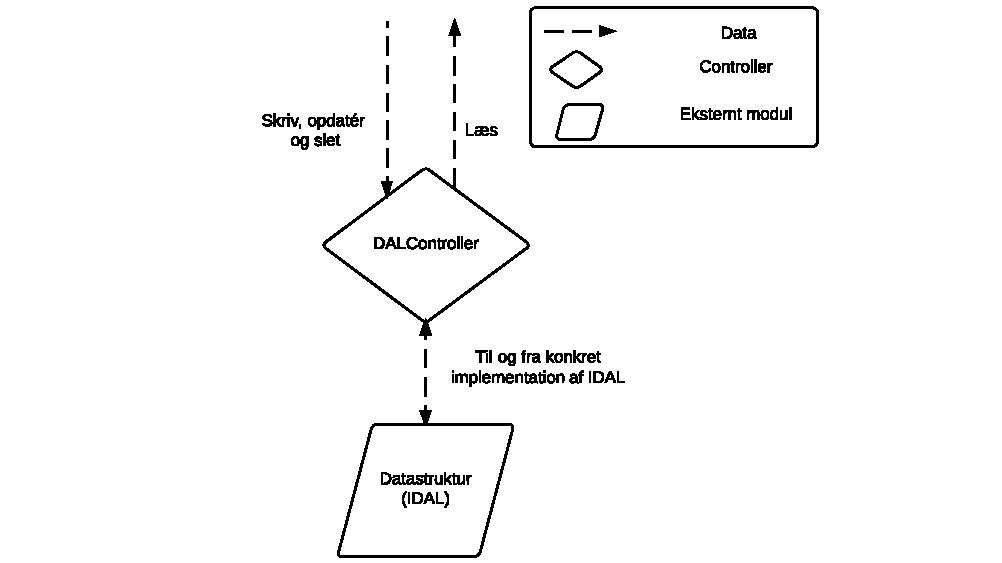
\includegraphics[width=\textwidth]{persistenslag-diagram.pdf}
  \caption{Diagram over persistenslagsmodulet}
  \label{fig:permod}
\end{figure}

Persistenslagsmodulet er opbygget således, at selve datastrukturen der manipuleres og læses fra, kan skiftes ud. Herved indkapsles tilgangen til datastrukturen. Dette gør det muligt, at programmet kan skifte fra benyttelse af xml-fil som datalager, til at benytte en database, uden at ødelægge anden eksisterende kode.

Som man kan se på \cref{fig:permod} består persistenslagsmodulet af én enkelt klasse, kaldet DALController. Denne klasse er kun bevidst om én konkret implementation af tilgangen til en datastruktur. Dette sker via interfacet IDAL. Når et andet modul ønsker at lave en CRUD operation på persistenslagsmodulet, videredelegeres denne operation, til den underliggende implementation af tilgangen til en datastruktur.
